% main.tex, to be used with thesis.tex
% This contains the main work of your thesis.

%\bibliography{thesis}  % uses the references stored in Chapter1Radar.bib

\chapter{Empirical Analysis of Data Persistence Taxonomies for NetBEAMS}

Providing data persistence for an existing sensor networks require analyzes of
the infrastructure and the nature of the produced data. Based on the taxonomies
of chapter 3, and the requirements of a data persistence for NetBEAMS in
chapter 4, this chapter aims at analyzing a group of database technologies
selected from literature review topics covered in chapter 2. Similarly,
supported by the scope of the required implementation presented in this
chapter, the comparison of the technogies is summarized, highlighting the
selected database system used for the design of a component for NetBEAMS and
used for the design of the experiments.

\section{Scope of the use of the Techonolgy}

The scope of the use of the database can involve different functional and
non-functional requirements defined in the last chapter. This work does not
intend to implement an application based on the database system selected, but
to provide the foundation of a database management system that can be used to
develop one focused in less refactoring and high scalability and performance.
For this reason, the use of the database system will be restricted to the data
persistence and use through native system or through the use of native
programming languages or API. In this way, the scope of this technology
selection can be summarized as follows:

\begin{itemize}
  \item Provide data management over the collected sensor data, as a
  conventional database system;
  \item Must be able to scale in the face of an increase to the data load of
  the sensor network, as described in chapter 2;
  \item  Must be able to use single or multiple servers to improve performance
  and optionally deal with Data-Centric approaches to sensor data partitioning;
  \item Must provide a data model that scales, decreasing the constant data
  schema changes.
\end{itemize}

\section{Database System ``Contenders''}

This section describes the database systems ``contenders'' considered to be used
as the persistence technology backend for NetBEAMS. As described in the
previous chapter, the selection of the technologies must be based on the list
of functional and non-functional requirements specified within the scope of
this work.

One of the essential questions related to data persistence is regarding the
data model and breed of the database. That is, the use of the relational or
any other model to describe data along with its management. Traditionally, the
relational data model has been used to provide data persistence for different
types of projects, inclusing sensor networks \cite{sn-dataware-house,
db-xml-enabled, sn-db-tinydb}. However, tradition does not always get translated
to efficiency in terms of problem solving. For this reason,
\cite{db-is-rdbs-dommed} reflects about the use of alternatives to the
relational model when the data persistence problem in consideration is to
provide data persistence for dynamic environments as Internet applications. The
author also suggests that the relational model is hard to maintain in
ever-changing environments, and thus, proposes the use of the Key-Value-Pair
(KVP) data model and a different number of technologies. Similarly,
\cite{cloud-comp-survey} reports similar trends in academic and industrial
research in distributed computing have used KVP databases in powerful systems
such as Cloud Computing \cite{cloud-comp-architectures}. For this reason, in
addition to the different database systems used by projects in the
literature review, this work also includes the review of a KVP database system
called mongoDB \cite{mongodb}, since it was among those cited in the surveys.
In such a manner, the list of the systems considered for assessment is the
following:

\begin{itemize}
  \item \textbf{MySQL}\cite{mysql}: system used in the implementation of a
  dateware house with sensor network data \cite{sn-dataware-house};
  \item \textbf{TinyDB}\cite{tinydb}: as referred in the literature review,
  TinyDB is a database system used in many different sensor networks
  implementation such as \cite{sn-db-tinydb};
  \item \textbf{MongoDB}\cite{mongodb}: an open-source KVP database
  system suggested by different surveys to be alternatives to relational
  databases \cite{db-is-rdbs-dommed, cloud-comp-architectures};
  \item \textbf{DB2}\cite{db2}: in the pursuit of an XML database system, DB2
  is listed as a hybrid database system that offers both the relational and the
  XML models \cite{db-xml-enabled}. Furthermore, it was selected because
  NetBEAMS represents serialized objects in XML, as shown in section
  \ref{sec:dsp-message}.
\end{itemize}

The following sections reviews these technologies' capabilities to adhere to
the specifications of the taxonomies defined in chapter 3, as well as the
requirements and the scope for a data persistence of NetBEAMS, as defined in
chapter 4.

\section{Analysis of the Purpose of Sensor Data}

The execution of the SF-BEAMS sensor network, together with the NetBEAMS
automated infrastructure, can be summarized as follows:

\begin{itemize}
  \item Data is generated by sensor devices, such as the YSI sonde
  \cite{YSI-Sonde}, and manually collected by using a laptop to the data sink
  at the RTC laboratories;
  \item Upon data reception, the RTC staff index and archive the data for
  distribution using the OPEnDAP format;
  \item An automated approach to the data collection procedures is performed 
  using NetBEAMS \cite{netbeams2009}, using software components to obtain and
  send the data to the data sink node. A complete description of this approach
  is detailed in section \ref{sec:netbeams-architecture}.
\end{itemize}

As summarized in the previous section, the nature of data from NetBEAMS through
SF-BEAMS is used for the purpose of \textbf{Data Archival}. After the
collected data captured from the sensors, it requires further processing
in order to be archived for later reuse. Different types of users are expected
to use the collected data, ranging from researchers, students, and the public 
over the Internet.

\subsection{Technology Analysis}

Since all of developed database systems were implemented with the intension of
persisting data in long-term storage devices, every single one in the list
provides support for data persistence and management. Therefore, they are
compliant to the purpose of Data Archival for the sensor networks.

\section{Analysis of the Location of Sensor Data}
\label{sec:sn-data-location}

As shown in the previous chapter, NetBEAMS's architecture is based on sensor
network whose topology is a single-hop star with a centralized data sink. In
this way, all the collected data is transmitted to that single location
\ref{sec:sn-infrastructure}. In the same vein, the simplest location to save
the collected data is through the use of at least an \textbf{External Storage}.
Similarly, the use of a Data-Centric Storage strategy is considered in
situations where the data sink is about to reach its storage capacity. As a
consequence, the \textbf{Data-Centric Storage} separates the collected data
into dissimilar locations, based on any property of the data. Therefore,
there are two different approaches to data partitioningThe two different
flavors: 

\begin{itemize}
  \item \textbf{Horizontal Partitioning}: the data segmentation is implemented
  based on the values of the table rows. That is, all the values defined by the
  columns are used in a given table physically located in specific servers.
  For instance, horizontal partitioning can be defined as a collection of five
  years worth of historical sensor data, partitioned into five separate
  servers. In this way, each server contains data related to each of the years;
  \item \textbf{Vertical Partitioning}: data is partitioned vertically in a way
  that the columns of an entity are divided into different database tables. In
  this way, the particular dataset is broken down to different tables. For
  example, if the database is used to store pictures of a given sensor camera
  in a BLOB column, it would be the most preferable to the scenario where the
  images are not constantly referenced when compared to the textual data.
\end{itemize} 

\subsection{Advantages of the External Storage Approach}

The External Storage approach is the most common way to implement persistence
for any breed of systems since data management is usually offered by most
database systems out-of-the-box. 

\subsection{Disadvantages of the External Storage Approach}

The most common problem related to a single External Data Storage is that 
resources may run into data management problems such reaching the disk storage
capacity or hardware failure.

\subsection{Advantages of the Data-Centric Approach}

The benefit of the Data-Centric approach can be directly associated with
database partitioning mechanisms described earlier. Since the collected data is
distributed into different locations, this approach decreases the size of
datasets when the database server performs a query processing in a database
table. For this reason, this approach helps the database administrators to
scale their database infrastructure and improve the database performance.

The horizontal or vertical partitioning strategies are also referred to as
Database Sharding \cite{db-shard-discussion}, or simply Database partitioning
\cite{db-partitioning-relational}. Both the former and the
latter are used in regular schema-dependent models or schema-less models,
which uses denormalized data models. There are different approaches to
partition data \cite{db-shard-schemas, db-partitioning-relational}.

\begin{itemize}
  \item \textbf{Directory Based Partitioning}: an ordinary lookup service is
  used to identify which database shard to use, where the lookup table can be
  stored in a secondary area;
  \item \textbf{Key or Hash Based Partitioning}: the value of a given key
  property can  be used as the key of the shard. Moreover, it can be used as 
  an input to a hash function, whose output determines at which database shard
  the data needs to be stored.
\end{itemize}

An example of a Data-Centric storage with different shards can be see in Figure
\ref{fig:database-sharding-by-region}, where the collected data is segregated
by its origin. Each shard is assumed to be placed in different server
hosts, as well as each of them uses the same ``denormalized'' data models.

\begin{figure}
  \centering
  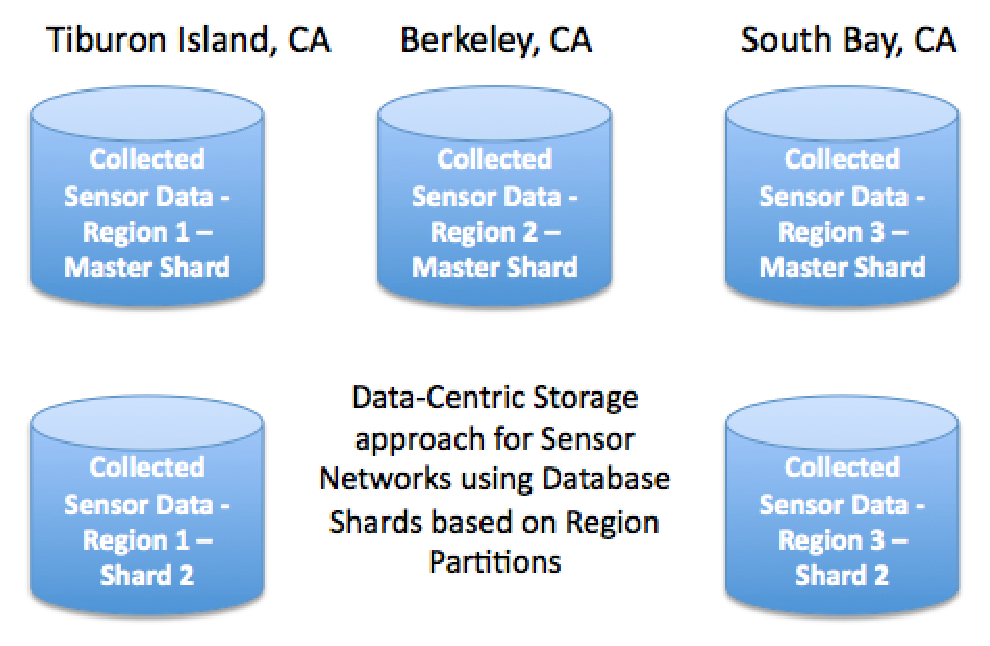
\includegraphics[scale=0.5]{../diagrams/database-sharding-by-region}
  \caption{Example of Data-Centric Storage for Sensor Networks using Database
  Sharding}
  \label{fig:database-sharding-by-region}
\end{figure}

\subsection{Disadvantages of the Data-Centric Approach}

The data partitioning is a highly restricted technology, normally available to
advanced users of distributed database systems. Despite being offered as a
common-off-the-shelf functionality by some popular database systems, this
strategy requires closer database management and configuration. Some of the
problems related to this strategy are regarding its lifecycle management
\cite{db-shard-discussion}:

\begin{itemize}
  \item \textbf{Rebalancing Shards}: considering a schema-dependent database
  system, changes on the schema of one shard requires rebalancing the
  collected data on each of the shards. As a consequence, the database shards
  transfers data to new locations whenever necessary. This technique is
  starting to appear as COTS implementations such as MySQL \cite{mysql} and
  mongoDB \cite{mongodb};
  \item \textbf{Referential integrity}: also considering a schema-dependent
  database system, any cross-shard query may fall into the problem where
  references do no exist in other shards, since the application layer is
  responsible for enforcing data integrity. In this way, examples of such
  include verifying constraints of foreign keys when the partition is done
  using Vertical table partitioning, considering that data collections are
  organized in separate spaces, and physically placed in different shard nodes
  \cite{db-partitioning-relational}.
\end{itemize}

\subsection{Technology Analysis}

\begin{itemize}
  \item \textbf{MySQL}: Supports External or Data-Centric Storage approaches.
  When Data-Centric Storage is used, both vertical and horizontal partitions
  \cite{db-partitioning-relational} can be chosen, using different strategies
  to partition the data;
  \item \textbf{TinyDB}: Only supports the External Storage;
  \item \textbf{MongoDB}: Supports External or Data-Centric Storage. When the
  latter approach is used, the horizontal partition strategy is available with
  automatic shards \cite{db-mongo-partition};
  \item \textbf{DB2}: Supports External and Data-Centric storage. Only supports
  vertical table partition for the data-centric storage \cite{db-db2-partition}.
\end{itemize}

All the selected database systems support the External Storage method. However,
they all differ with the support to Data-Centric Storage support. Therefore,
MySQL and mongoDB are promising choices, with the difference of the use of the
data model.

\section{Analysis of the Data Model}

One of the most common practices in the area of database system is to use the
relational model to persist data, although the application of the system may
not fit to solve the problem. In fact, the main users of sensor networks may
not possess any expertise in database systems or data modeling, based on the
fact that they are from different science areas. \cite{sn-programming-language}
suggested the use of programming languages abstraction instead of regular
database systems for researchers. For instance, SF-BEAMS is managed by Marine
Biologists without expertise in Data Management, Modeling systems, and for
this reason, one of the requirements of the system is trying the use of
schema-less approaches. The \textbf{Key-Value-Pair Data Model} or the
\textbf{Document-Oriented Data Model} seems to be the simplest choices of the
models.

\subsection{Analysis of the Schema-Dependent Models}

Considering the inception of a relational data model \cite{relational-model}
and the use of the YSI Sonde data as the main entity in the system, let Figure
\ref{fig:Relational-Model-Original} represent a prototype of the relational 
model, after passing through the process of normalization
\cite{db-normalization}.

\begin{figure}
  \centering
  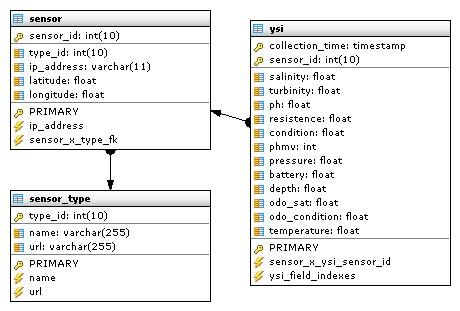
\includegraphics[scale=0.5]{../diagrams/Relational-Model-Original}
  \caption{Relational Data Model for NetBEAMS - A first prototype}
  \label{fig:Relational-Model-Original}
\end{figure}

Supposing a new type is added into the system, let the refactored version of
the relational model be depicted in Figure
\ref{fig:Relational-Model-Addition-Modified}. Some observations are
considered in this scenario:

\begin{figure}
  \centering
  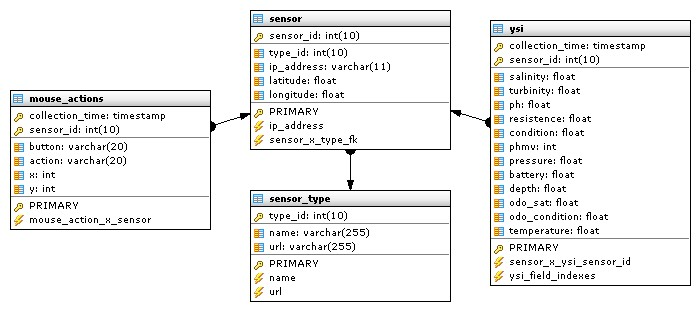
\includegraphics[scale=0.5]{../diagrams/Relational-Model-Addition-Modified}
  \caption{Relational Data Model for NetBEAMS - Modified version with new
  entity}
  \label{fig:Relational-Model-Addition-Modified}
\end{figure}

\begin{itemize}
  \item Data schema that constantly changes require constant database
  normalization processes, changes to structure, database management, and all
  the code that uses the data. Schema-Dependent databases always require
  refactoring of the schema to accommodate changes to the entites' properties;
  \item The approach of Relational Model might not fit the nature of the
  collected data from sensor devices, since they tend to change over time. 
  Furthermore, the support to time-series or provenance are not better
  supported \cite{sn-provenance};
  \item Some research have suggested changes to the SQL clauses to better
  support time-series when collecting data using the relational model 
  \cite{sn-db-newop}.
\end{itemize}

Other projects have used the XML data models for persistence. It falls
into the same category as the Relational Model using XML documents \cite{xml},
since XML documents must fulfill the specifications defined by an XML Schema
\cite{xml-schema}. This model uses XPath \cite{xml-xpath} technology for
querying documents, although some hybrid \cite{db2} technologies may still use
SQL \cite{sql} for that matter. In this way, a materialized version of the
data from the defined previous schema can be seen in Figure
\ref{fig:persistence-example-relational}.

\begin{figure}[!h]
  \centering
  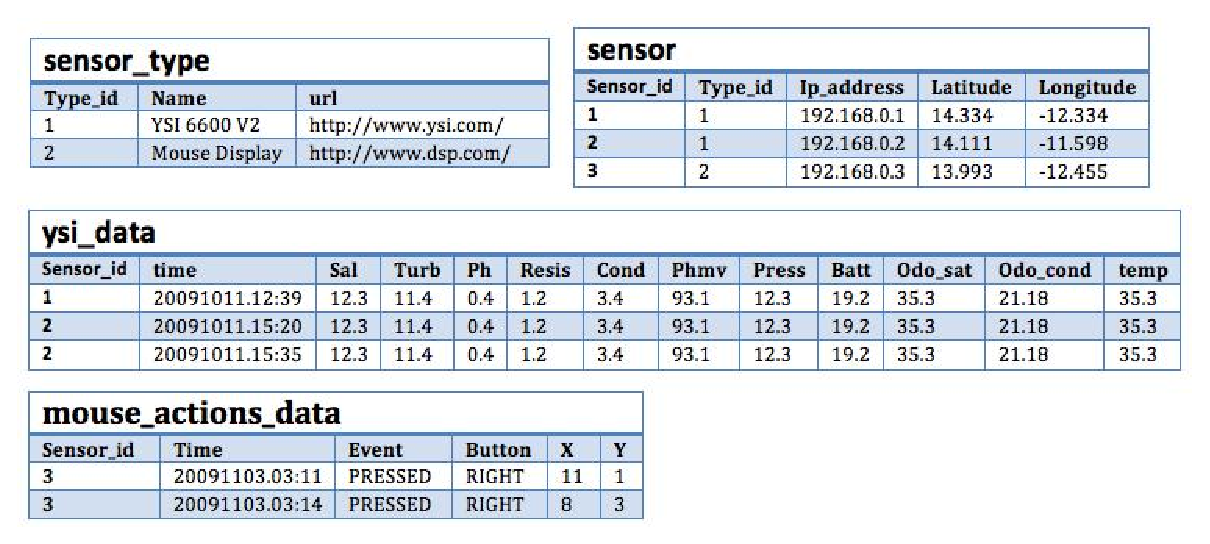
\includegraphics[scale=0.7]{../diagrams/persistence-example-relational}
  \caption{Instance of a Relational Model Database Prototype}
  \label{fig:persistence-example-relational}
\end{figure}

Although this data model has been used in different types of applications,
developers have tried to use the Relational Model to design an application that
could prevent any database change through the use of a technique that relates a
key to a value, called Key-Value data model. As mentioned earlier, with the
emergence of Internet applications, the necessity of such a model that does
not require constant refactoring led developers to propose such manner using
the relational model as documented in technical articles such as
\cite{db-kvp-in-relational01} and \cite{db-kvp-in-relational02}. Based on
these articles, consider the relational model depicted in Figure
\ref{fig:KVP-on-Relational-Model} as a data model for persisting data to our
case study using the key-value strategy. It is clear that this approach
contains problems: repetition occurs, since the nature of
time-series data requires the use of a timestamp key for each property of the sensor. Therefore, this strategy is not
well-suited to provide persistence data from collected sensor networks.

\begin{figure}[!h]
  \centering
  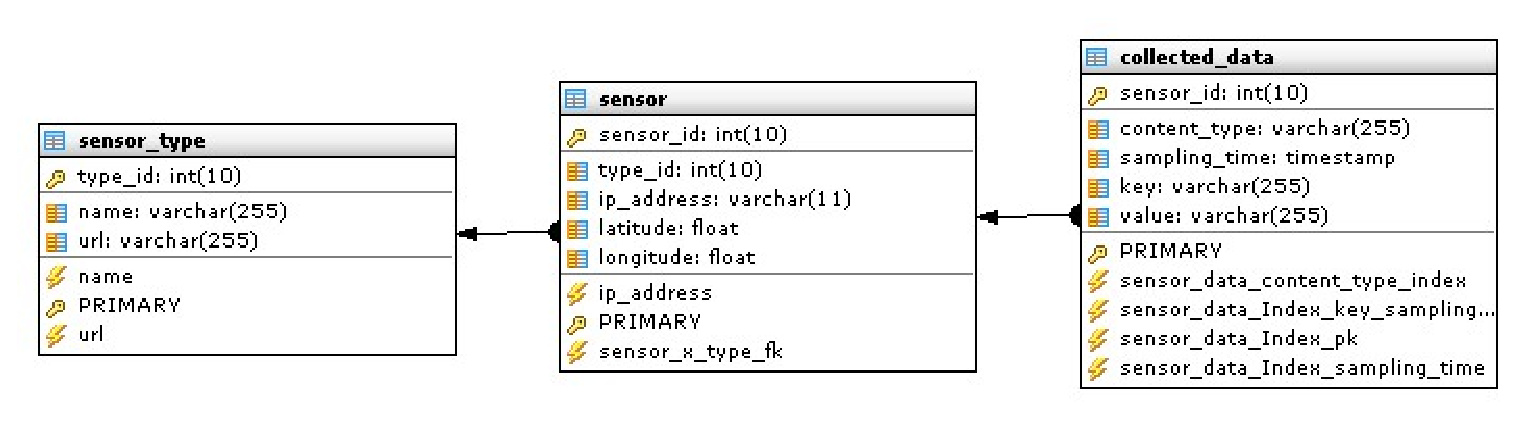
\includegraphics[scale=0.6]{../diagrams/KVP-on-Relational-Model}
  \caption{KVP Data Model implementation using Relational Model}
  \label{fig:KVP-on-Relational-Model}
\end{figure}

\begin{figure}[!h]
  \centering
  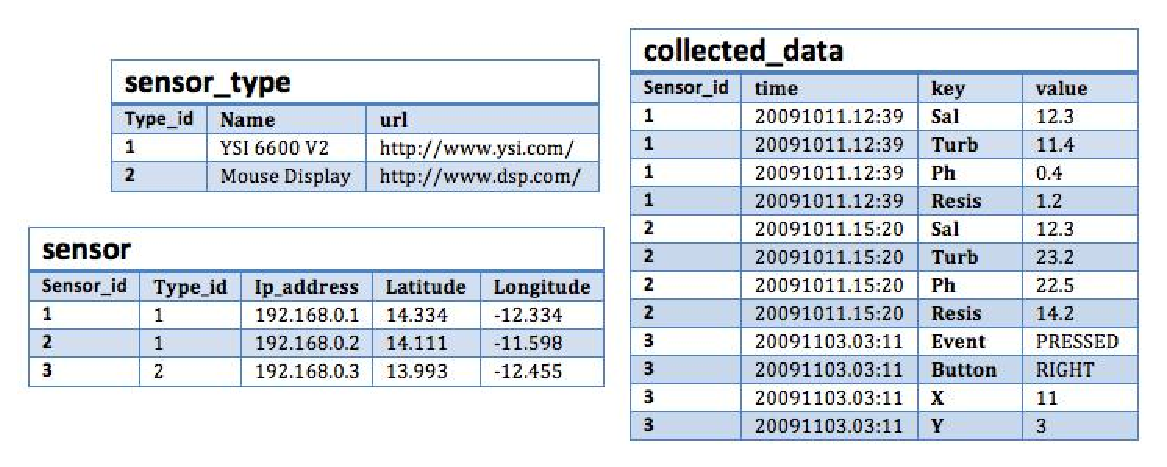
\includegraphics[scale=0.75]{../diagrams/persistence-example-relational-kvp}
  \caption{KVP over Relational Model Database Prototype}
  \label{fig:persistence-example-relational-kvp}
\end{figure}

\subsection{Analysis of the Schema-less Models}

The growth of distributed systems and the Internet have enabled the development
of powerful database servers that can be organized in the context of
infrastructure and how to represent models. A powerful up-coming approach is
the use of database systems that do not use structured language for querying
its data. One such example is called Key-Value Pair (KVP) data model
\cite{db-kvp}, which is also known as Document-Oriented, Distributed Hash
Table. Such a model has the following properties:

\begin{itemize}
  \item data is structured in collections of key-value pairs, as it is done in
  hash data structure. The definition of the key is a given property with its
  associating value;
  \item the query process is using mechanics similar to programming or
  scripting language, that is, the use of APIs in a given programming language.
\end{itemize}

There are no records of the use of this data model with Sensor Networks.
Different variants of such data model is the document-oriented data model,
where data is modeled using structured documents. However, these documents
have a dynamic structure, freely described without the use of a
schema validation mechanism as used in XML Schema. One example of such
approach is the use of the JSON data format \cite{json}. mongoDB implements the
following:

\begin{itemize}
  \item entities from the same domains are placed into a ``bucket'';
  \item entities have a set of attributes and relating values
  \item entities with different set of attributes may be contained in the same
  bucket, since there is no schema to govern the bucket items restriction.
\end{itemize}

For instance, all data needed for the YSI sonde data, as well as all necessary
provenance data that describes the data, depicted in section
\ref{sec:sn-data-description}, are represented by means of key-value pairs
\ref{fig:persistence-example-kvp}.

\begin{figure}[!h]
  \centering
  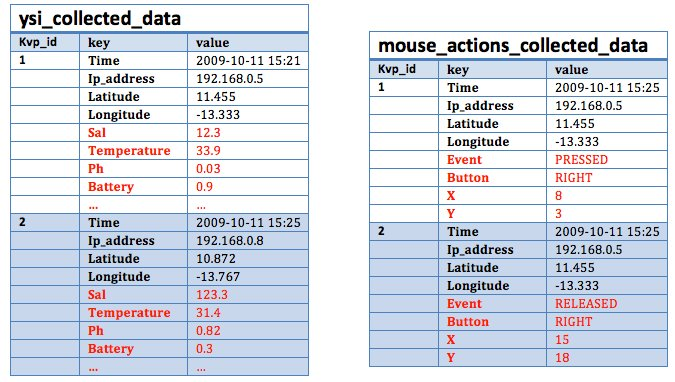
\includegraphics[scale=0.5]{../diagrams/persistence-example-kvp}
  \caption{KVP Database instance Prototype}
  \label{fig:persistence-example-kvp}
\end{figure}

\subsection{Technology Analysis}

The relational and key-value data models were compared by
\cite{db-is-rdbs-dommed} and is compared on table
\ref{tab:schema-vs-schemaless}:

\begin{table}
    \label{tab:schema-vs-schemaless}
    \caption{Schema-Dependent X Schema-less Databases Compared: Properties}
    \begin{center}
    \begin{tabular}{|p{210pt}|p{210pt}|}\hline
    Schema-Dependent Databases & Schema-less Databases\\\hline
    \begin{enumerate}
      \item Real-world model represented by entities, classified in tables;
      \item Tables composed by columns and rows. Rows are comprised by column
      values, which have the same schema;
      \item Data Model is defined in advance with a schema, which contains
      relationships and constraints to enforce data integrity;
      \item Data represents ``natural'' entities, not application specific;
      \item Data Normalization is the data structuring process to remove data
      duplication, as well as establishing data associations through table
      relationships \cite{db-normalization};
      \item Data Provenance can be provided through data types such as
      ``Timestamp'' for time or float for the GPS float-based coordinates; 
    \end{enumerate} 
    & 
    \begin{enumerate}
      \item Real-world model by entities, classified in Domains;
      \item Domains are similar to tables, but like buckets that contains items
      without a pre-defined schema, what enable them to have different schemas;
      \item Items are identified by keys, as well as have a dynamic set of
      attributes attached to it, however with no schema defined;
      \item Items may represent not only the natural representation of data, but
      also include application-specific data;
      \item Since data may be repeated, no data normalization is done, so that
      integrity is done in the application layer;
      \item Data provenance can be added through the use of keys and relating
      values for the time information and location of the data.
    \end{enumerate}
    \\\hline
    \end{tabular}
    \end{center}
\end{table}

\begin{table}
    \label{tab:schema-vs-schemaless-daccess}
    \caption{Schema-Dependent X Schema-less Databases: Data Access}
    \begin{center}
    \begin{tabular}{|p{210pt}|p{210pt}|}\hline
    Schema-Dependent Databases & Schema-less Databases\\\hline
    \begin{enumerate}
      \item The basic operations CRUD\footnote{Create-Retrieve-Update-Update
      database operations} data are performed using a structured language such
      as the SQL or XPath;
      \item Query languages can access data from different tables through
      joins, contains functions for aggregation and complex filter.
    \end{enumerate} 
    & 
    \begin{enumerate}
      \item The CRUD operations are performed via API\footnote{Application
      Programming Interface} through programming languages;
      \item Some technologies provide basic SQL-like syntax for filter criteria
      with some predicates like =, !=, <, > that ca be applied;
      \item The data and application integrity logic is placed in the
      application layer.
    \end{enumerate}
    \\\hline
    \end{tabular}
    \end{center}
\end{table}

\begin{table}
    \label{tab:tab:schema-vs-schemaless-api-interface}
    \caption{Schema-Dependent X Schema-less Databases: Application Interface}
    \begin{center}
    \begin{tabular}{|p{210pt}|p{210pt}|}\hline
    Schema-Dependent Databases & Schema-less Databases\\\hline
    \begin{enumerate}
      \item Have their own specific API or through ODBC\footnote{Open Database
      Connectivity};
      \item Data is stored in a format that represents its natural structure,
      and for this reason, in a single or distributed fashion.
    \end{enumerate} 
    & 
    \begin{enumerate}
      \item Systems tend to provide SOAP/REST \cite{http-rest};
      \item \cite{db-is-rdbs-dommed} claims that data is stored in a more
      effective way, requiring only code plumbing for the relational code;
    \end{enumerate}
    \\\hline
    \end{tabular}
    \end{center}
\end{table}

Since the selected data model is the schema-less one, the following can be seen
from the technologies:

\begin{itemize}
  \item \textbf{MySQL}: supports the Relational Data Model;
  \item \textbf{TinyDB}: supports the Relational Data Model; 
  \item \textbf{MongoDB}: supports Key-Value Pair Data Model;
  \item \textbf{IBM DB2}: supports the Relational Model and the Structured
  Data models.
\end{itemize}

\section{Analysis of the Data Description}

\textbf{Data Description} is the methods used to describe the collected data
from sensors, specially those produced by real-time data streams. Since those
type of data does not include descriptions of its values, data provenance
offers guidelines to improve the description of the collected data.

An additiona to data provenance, annotations is another technique used to
better describe the collected data from sensor devices. Its main purposes is to
provide means of identifying observations, creating indexes based on simple
keywords. For an environmental sensor networks, this is a valuable type of value
used to better manage the collected data.

\subsection{Advantages of the Provenance-Aware Data}

The injection of provenance data into the collected data enriches description
of a given event, and is always useful to determine different aspects of the
data. As mentioned in chapter 3, data provenance helps identifying the nature
of the data by the identification of the properties of a given sensor device,
for example. Similarly, provenance adds spatio-time data in order to correlate
the observed data with time a given location and time of occurrence.

\subsection{Disadvantages of the Provenance-Aware Data}

Additional data being inserted together with the raw data collected from the
sensor devices. This additional data may contribute with any decreasing number
of disk storage for the variable defined. Therefore, the decreasing amount
of disk space may be one the reasons to not use annotations.

\subsection{Advantages of the Annotations}

Annotations are used to describe the collect data even more, since the
additional ``notes'' of the data are being stored together with the data. For
example, the use of tags to a given entity may help identifying and different
observations regarding the data collected from sensor devices.

\subsection{Disadvantages of the Annotations}

This type of data does not make part of the collected data, nor provenance
information. 

\subsection{Technology Analysis}

All the database systems technology supports the use of Data Provenance or
Annotations. The Key-Value Pair data model has the advantage of not maintaining
a schema design, and therefore, can add any type of data, and therefore,
mongoDB is the lead in this taxonomy.

\section{Analysis of the Query Processing Mechanism}

As a direct result from the previous section, the use of \textbf{Centralized Query
Processing} is indicated for NetBEAMS, also given the fact that SF-BEAMS data
goes directly to the individual network sink and, therefore, a centralized
point of the data.

\subsection{Advantages of the Centralized Query Processing}

Centralized data management and query processing is simpler than the in-network
query method. Data is verified by a straightforward database management system
without the risk of data being unavailable, when the data is spread among the
network nodes.

\subsection{Disadvantages of the Centralized Query Processing}

When the Centralized Query processing is used, problems may occur. Depending on
the size of the datasets and the database technology, performance may be a
concern. For example, this procedure creates of the alleged Funneling Affect
\cite{sn-storage04}, since the point-of-traffic is concentrated in the
centralized system.

In order to mitigate the problems originated by this query processing
mechanism, techniques such as Data Replication can be used.

\subsection{Technology Analysis}

All the database systems technology support a centralized query system. In
addition to that, they can be distributed into different distributed nodes when
used in a partioned environement.

\section{Analysis of the System Organization}

Sensor Network data can be saved in either Centralized or Distributed Systems.
While Centralized Database Systems are easier to manage, it may
face challenges regarding its data. In order to implement a Data-Centric
solution, a distribute database system must be in place in order to manage
the different data by a single node.

\subsection{Advantages of Database Partitioning}

\begin{itemize}
  \item Data-Centric queries and data use;
  \item Solves bottleneck problems related to reads/writes;
  \item Decrease the funneling effect by directing queries to given data
  partition;
\end{itemize}

\subsection{Disadvantages of Database Partitioning}

\begin{itemize}
  \item Very advanced topics in Database System;
  \item Partitions need to be rebalanced in case the key of the selected 
  partitioning strategy is changed.
\end{itemize}

\subsection{Technology Analysis}

\begin{itemize}
  \item \textbf{MySQL}: Supports Data Replication;
  \item \textbf{TinyDB}: NO Supports to distributed data;
  \item \textbf{MongoDB}: Supports Data Replication;
  \item \textbf{IBM DB2}: Supports Data Replication.
\end{itemize}

\section{Other Non-Functional Analysis}

\begin{itemize}
  \item \textbf{Open-source}: Given the fact of the nature of the project, the
  technology to be used must be free of charge \cite{open-source}, that is, no
  costs involved in the adoption a such technology; Together with it is the
  support from the community;
  \item \textbf{Native APIs}: In order to consider the scope of this work
  defined in the last chapter, the solution for persisting collected sensor
  data must be not only limited to a technology that provides data access, such
  as SQL, but also by other data access mechanisms \textbf{data access
  mechanisms};
  \item \textbf{Hot Backup}: Supports hot backup with less service interruption. 
\end{itemize}

\subsection{Technology Analysis}

Most of the technologies listed provides access to the data sets through the
use of drivers in different programming and scripting languages such as Java,
Python, Perl, among others. Moreover, only TinyDB does not support hot backup.

\begin{itemize}
  \item \textbf{MySQL}: Is  open-source, supports hot backup and contains
  scripting APIs from  the community;
  from the community. Also APIS are available for the majority of languages;
  \item \textbf{TinyDB}: Not open-source;
  \item \textbf{MongoDB}: An open-source database system with an increasing
  support from  the community, offering native APIS in different programming
  languages and scripting languages;
  \item \textbf{IBM DB2}: Not Open-Source, but offers support from its
  community.
\end{itemize}

Only MySQL and MongoDB supports the non-functional requirements defined in this
section.

\section{Global Analysis Results and Technology Selection}

Each of the databases were scored according to its support to the different
types of taxonomies, as well as a different set of requirements. As defined
in the scope of the database system, the database that can provide a
programming language abstracton to its data access would be selected.
Moreover, the database technology should offer the support to schema-less
databases. As a result, mongoDB was selected because of different reasons.
First, it is a document-oriented database system, which does require the use of
SQL languages. Similarly, it had been reported in two different surveys as
potential database systems. Finally, there were no references in the literature
regarding the use o KVP databases in sensor networks, and for this reason, this
proposal was performed, supporting most of the taxonomies defined in the
previous chapter, it was selected for the implementation of the DSP Data
Persistence component for NetBEAMS.

\begin{table}
    \label{tab:technology-selection}
    \begin{center}
        \begin{tabular}[!h]{|c|c|c|c|c|c|c|}\hline 
        \textbf{Database} & \textbf{MySQL} & \textbf{TinyDB} & \textbf{MongoDB} & \textbf{IBM DB2}\\\hline
        Centralized Query & + & + & + & + \\\hline 
        Distributed System & ++ & - & ++ & +\\\hline 
        Schema-less & - & - & + & -\\\hline 
        Provenance Support & + & + & + & +\\\hline 
        NO-SQL Query & - & - & + & -\\\hline 
        Partition & + & - & + & +\\\hline 
        Export Capability & + & - & + & -\\\hline 
        Programming Language. & + & + & + & +\\\hline
        Script Language. & + & - & + & +\\\hline
        Open-Source & + & + & + & -\\\hline
        \end{tabular}
        \caption{Technologies Selection Grading}
    \end{center}
\end{table}

To conclude, this chapter evaluated different database systems selected from
the literature reviews of chapter 2. After presenting the database system
``contenders'', the analysis of each of the taxonomies were conducted for each
of the technologies, culminating with the technology selection comparison. In
this way, the following chapter describes the design of the solution using
mongoDB as the primary solution for the backend.
